\section{Chapter 11: Quivers and path algebras}\label{sec:14-appendix-solutions:10-chapter-11:1}

\textbf{1. Adding a cycle}

\begin{lstlisting}
inductive CyclicArrow where
  | alpha : CyclicArrow   -- 0 (*$\rightarrow$*) 1
  | beta : CyclicArrow     -- 1 (*$\rightarrow$*) 2
  | gamma : CyclicArrow    -- 2 (*$\rightarrow$*) 0

def cyclicQuiver : Quiver (Fin 3) CyclicArrow where
  source := fun a => match a with
    | CyclicArrow.alpha => 0
    | CyclicArrow.beta => 1
    | CyclicArrow.gamma => 2
  target := fun a => match a with
    | CyclicArrow.alpha => 1
    | CyclicArrow.beta => 2
    | CyclicArrow.gamma => 0

def cPathAlpha : Path cyclicQuiver 0 1 :=
  Path.cons CyclicArrow.alpha rfl rfl (Path.nil 0)

def cPathBetaAlpha : Path cyclicQuiver 0 2 :=
  Path.cons CyclicArrow.beta rfl rfl cPathAlpha

def cPathGammaBetaAlpha : Path cyclicQuiver 0 0 :=
  Path.cons CyclicArrow.gamma rfl rfl cPathBetaAlpha
\end{lstlisting}

Each \href{https://lean-lang.org/doc/reference/latest/Tactic-Proofs/Tactic-Reference/}{\texttt{rfl}} again discharges a source/target proof obligation that reduces, by definition, from the \texttt{match} in \texttt{cyclicQuiver}. Observe that \texttt{cPathGammaBetaAlpha} is a nontrivial loop at vertex \texttt{0}. The path algebra of a quiver with cycles has elements of arbitrarily high ``length,'' which is exactly why such algebras are usually infinite-dimensional unless relations (an ``admissible ideal'') are imposed on the path algebra.

\textbf{2. \texttt{theorem append\_\allowbreak{}nil\_\allowbreak{}left}}

\begin{lstlisting}
theorem append_nil_left {V A : Type} {Q : Quiver V A} {u v : V} (p : Path Q u v) :
    Path.append (Path.nil u) p = p := by
  induction p with
  | nil =>
    -- Goal: Path.append (Path.nil u) (Path.nil u) = Path.nil u
    -- (`nil`'s case binds no fresh variable here (*\textemdash{}*) the vertex is already
    -- fixed by p's own type (*\textemdash{}*) so there is nothing to name.)
    -- Path.append unfolds on its second argument being `nil`, giving
    -- `Path.nil u` on the nose.
    rfl
  | cons a h h' q' ih =>
    -- ih : Path.append (Path.nil u) q' = q'
    -- Goal: Path.append (Path.nil u) (Path.cons a h h' q') = Path.cons a h h' q'
    show Path.cons a h h' (Path.append (Path.nil u) q') = Path.cons a h h' q'
    rw [ih]
\end{lstlisting}

This is exactly what the editor shows in the \texttt{cons} case: the Lean Infoview lists every hypothesis the pattern match introduces --- \texttt{Q : Quiver V A}, \texttt{h : Q.source a = v}, \texttt{h' : Q.target a = wt}, \texttt{q' : Path Q u vt}, and the induction hypothesis \texttt{ih : (Path.nil u).append q' = q'} --- above the line, with the goal \texttt{(Path.nil u).append (Path.cons a h h' q') = Path.cons a h h' q'} below it:

\begin{figure}
\centering
\pandocbounded{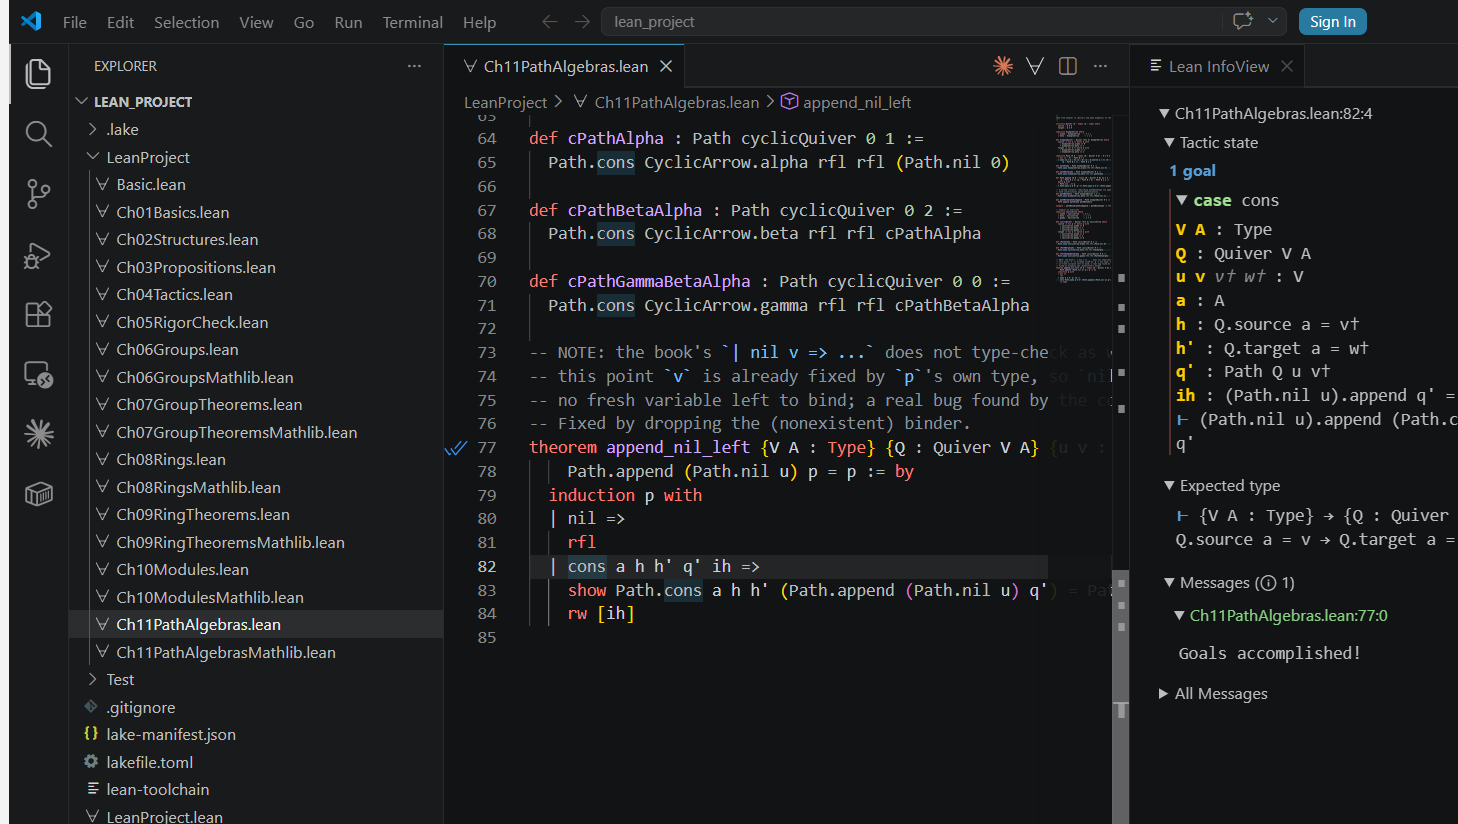
\includegraphics[keepaspectratio,alt={The Lean Infoview panel in VS Code, showing the tactic state for the cons case of append\_nil\_left's induction: hypotheses V A : Type, Q : Quiver V A, u v vt wt : V, a : A, h : Q.source a = v, h\textquotesingle{} : Q.target a = wt, q\textquotesingle{} : Path Q u vt, ih : (Path.nil u).append q\textquotesingle{} = q\textquotesingle, and the goal (Path.nil u).append (Path.cons a h h\textquotesingle{} q\textquotesingle) = Path.cons a h h\textquotesingle{} q\textquotesingle.}]{../14-appendix-solutions/../11-path-algebras/images/append-nil-left-infoview.png}}
\caption{The Lean Infoview panel in VS Code, showing the tactic state for the \protect\texttt{cons} case of \protect\texttt{append\_\allowbreak{}nil\_\allowbreak{}left}'s induction: hypotheses \protect\texttt{V A : Type}, \protect\texttt{Q : Quiver V A}, \protect\texttt{u v vt wt : V}, \protect\texttt{a : A}, \protect\texttt{h : Q.source a = v}, \protect\texttt{h' : Q.target a = wt}, \protect\texttt{q' : Path Q u vt}, \protect\texttt{ih : (Path.nil u).append q' = q'}, and the goal \protect\texttt{(Path.nil u).append (Path.cons a h h' q') = Path.cons a h h' q'}.}
\end{figure}

This mirrors \texttt{Path.append}'s own recursion, case for case. \texttt{Path.append} was defined by matching on its second argument, so \texttt{induction p} (which splits into cases on exactly that argument, generating the matching induction hypothesis \texttt{ih} in the \texttt{cons} case) unfolds the definition directly. In the \texttt{nil} case, both sides are \texttt{Path.nil u} by definition. In the \texttt{cons} case, unfolding \texttt{Path.append}'s defining equation turns the goal into \texttt{Path.cons a h h' (Path.append (Path.nil u) q') = Path.cons a h h' q'} (the \href{https://lean-lang.org/doc/reference/latest/Tactic-Proofs/Tactic-Reference/}{\texttt{show}} line makes this explicit rather than leaving it to elaboration), and \texttt{rw [ih]} completes the proof using the induction hypothesis.

\textbf{3. Sketch of \texttt{PathAlgebra}}

\begin{lstlisting}
-- A k-linear combination of paths from u to v, as a finitely-supported
-- function from paths to coefficients. `Finsupp`-style support tracking is
-- the honest way to do this; a simplified sketch:
structure PathAlgebraElem (V A : Type) (Q : Quiver V A) (k : Type) where
  -- coeff p = the coefficient of path p, for finitely many nonzero p
  coeff : {u v : V} (*$\rightarrow$*) Path Q u v (*$\rightarrow$*) k
  -- (a finiteness/support condition would be required here in a full
  -- development, e.g. via Mathlib's `Finsupp`)

-- To satisfy `Ring` (Chapter 8), `PathAlgebraElem` would need:
--   addGrp : CommGroup (PathAlgebraElem V A Q k)   -- pointwise addition of coefficients
--   mul    : concatenate paths, multiplying and summing coefficients over
--            all ways two paths compose (zero when endpoints don't match)
--   one    : the sum, over all vertices v, of 1 (*$\cdot$*) (trivial path at v)
--            (an idempotent identity, since Q may have infinitely many
--            vertices this "one" is only literally an element when Q0 is
--            finite (*\textemdash{}*) for infinite Q the path algebra is typically only
--            a "ring with local units," a subtlety Mathlib's category-
--            theoretic treatment handles more gracefully than a bare Ring)
\end{lstlisting}

The real finiteness/support bookkeeping (tracking which paths have nonzero coefficient) is exactly what makes a full formalization a genuine project rather than a one-page exercise. This sketch identifies the three \texttt{Ring} fields that require it (\texttt{addGrp}, \texttt{mul}, \texttt{one}), and shows why \texttt{one} is the subtle one when \(Q_0\) is infinite.

\textbf{Checkpoint project: path length, and composition respects it}

\begin{lstlisting}
def Path.length {V A : Type} {Q : Quiver V A} : {u v : V} (*$\rightarrow$*) Path Q u v (*$\rightarrow$*) Nat
  | _, _, Path.nil _ => 0
  | _, _, Path.cons _ _ _ p => p.length + 1

theorem Path.append_length {V A : Type} {Q : Quiver V A} {u v w : V}
    (p : Path Q u v) (q : Path Q v w) :
    (Path.append p q).length = p.length + q.length := by
  induction q with
  | nil =>
    simp only [Path.append, Path.length]
    rw [Nat.add_zero]
  | cons a h h' q' ih =>
    simp only [Path.append, Path.length]
    rw [ih, Nat.add_assoc]

example : (Path.append pathAlpha pathBetaOnly).length =
    pathAlpha.length + pathBetaOnly.length :=
  Path.append_length pathAlpha pathBetaOnly

#eval pathAlpha.length                                    -- 1
#eval pathBetaAlpha.length                                -- 2
#eval (Path.append pathAlpha pathBetaOnly).length          -- 2
\end{lstlisting}

\texttt{Path.length} recurses on the same two constructors as \texttt{Path.append} itself (§4--§5): \texttt{nil} contributes \texttt{0}, and each \texttt{cons} adds one to the length of the shorter path it extends. The proof of \texttt{append\_\allowbreak{}length} mirrors \texttt{Path.append}'s own recursion case for case, exactly as the project asked, but with one genuine surprise if \texttt{rfl} is tried first in either case: it fails. \texttt{Path} is \emph{indexed} by both endpoints. Because of this, Lean compiles a match on an indexed family so that its defining equations reduce only through their auto-generated equation lemmas, not through plain iota-reduction, once an abstract path (\texttt{p}, \texttt{q'}) is involved. Concrete, fully closed paths like \texttt{pathAlpha} still reduce fine under \texttt{\#eval} --- that is why the three checks above work directly. But the \emph{general}, universally-quantified theorem does not close by \texttt{rfl}. \texttt{simp only [Path.append, Path.length]} names exactly the two definitions being unfolded and nothing else, so it plays the same explicit role a \texttt{rw} would if these equations were reachable that way --- it is not standing in for an unknown pile of simp lemmas, only for the two named here. This is the same kind of real, verified obstacle Chapter 6 §4's \texttt{Perm3.ext} ran into with core Lean's lack of a \texttt{structure} extensionality lemma, now met again with indexed recursion instead.
